% !TEX root = ../thesis-example.tex
%

\chapter{ARCH/GARCH Volatility Models}

\section{ARCH}

An ARCH (autoregressive conditionally heteroscedastic) model is a model for variance of time series. ARCH models are used to descirbea changing, possibly volatility varance. models were created in the context of econmetric and finance problems having to do with the amount that investments or stock increases (or decrease) per time period, so there's a tendency to descibe them as models for that type of variable. For that reason, the variable of interests will be log returns. 

\begin{figure}[!h]
	\centering
	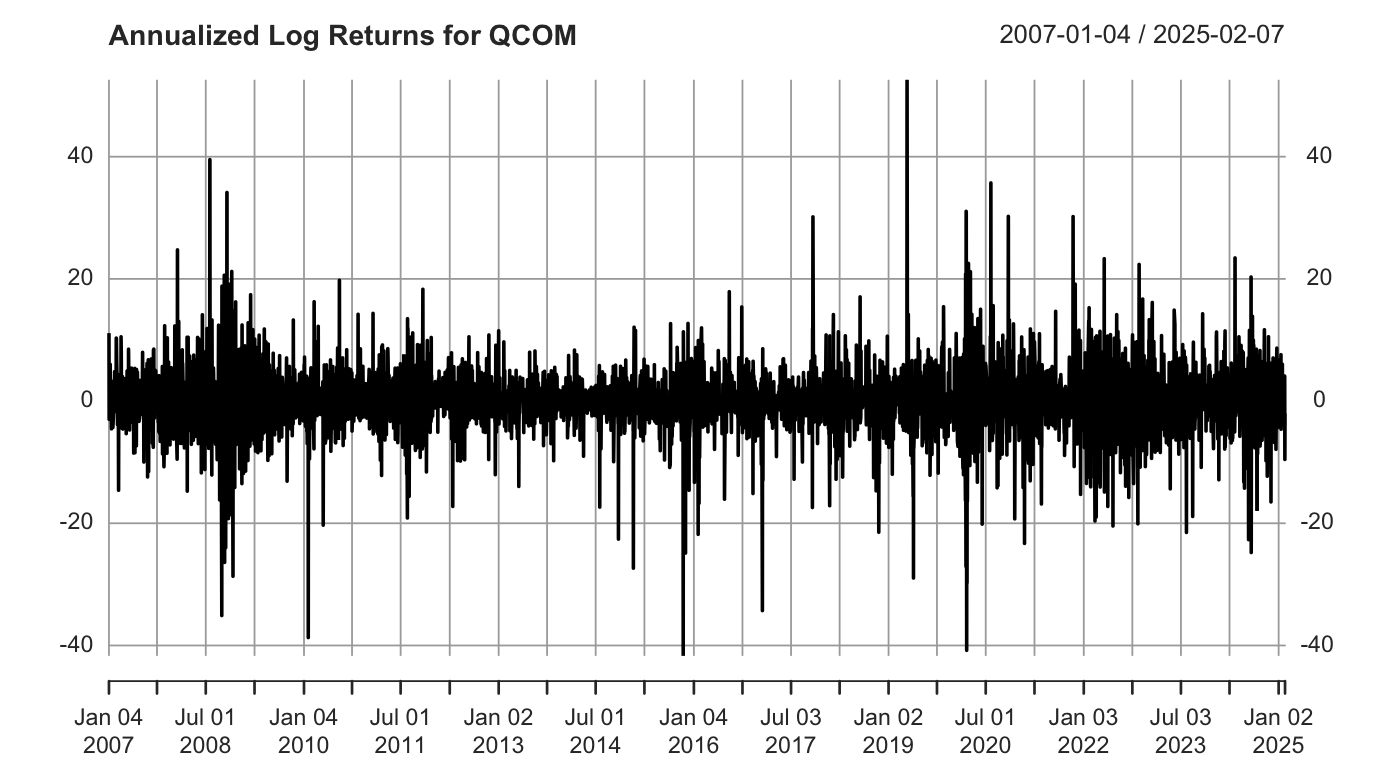
\includegraphics[width=0.8\linewidth]{content/plots/qcom_log_returns.png}
	\caption{Annaulized Logged Returns of QCOM}
	\label{fig:qcom_returns}
\end{figure}

The ARCH(1) model for the variance of model $r_t$ is that conditional on $r_{t-1}$, the variance at time $t$ is 
\begin{equation}
	\text{Var}\left(r_t|r_{r_{t-1}}\right)=\sigma_t^2=\alpha_0+\alpha_1r_{t-1}^2\quad 
\end{equation}

Figure (\ref{fig:qcom_returns}) shows the annualized log returns for QCOM  from January 4, 2007, to February 7, 2025. The returns are highly volatile, with pronounced spikes-both positive and negative-especially noticeable during periods like the 2008 financial crisis and the COVID-19 pandemic in 2020. Overall, the data oscillates around zero, reflecting frequent fluctuations in QCOM’s stock returns over the observed period. An ARCH model could be used for any series that has periods of increased or decreased variance. This might, for example, be a propery of residuals after an ARMA or ARIMA model has been fir to the data. As such, we will use the ARMA(2,2) that we have built earlier.

\begin{figure}[!h]
	\centering
	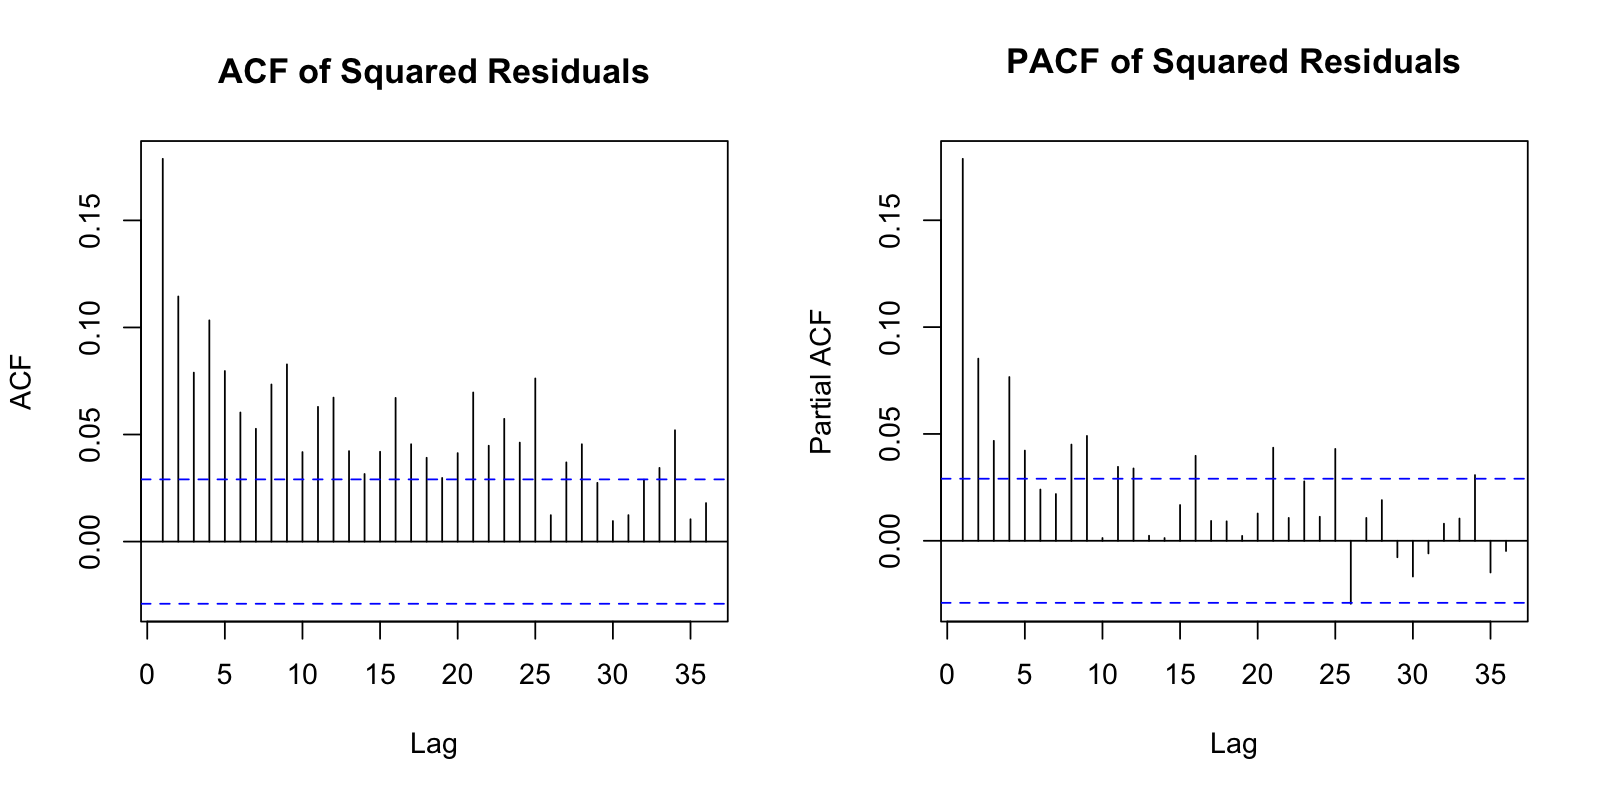
\includegraphics[width=0.85\linewidth]{content/plots/ACF_PACF_squared_residuals_QCOM.png}
	\caption{ACF and PACF of the Squared Residuals of ARMA(0,2)}
	\label{fig:ACF_PACF_residuals_QCOM}
\end{figure}

Figure (\ref{fig:ACF_PACF_residuals_QCOM}) displays the ACF/PACF in the ARMA(2,2) model residuals. For the ACF plot, we see multiple significant autocorrelations that extend well above the signficance bounds. The first several lags (particularly lags 1-5) show strong positive autocorrelation. There is also persistence of significant spikes throughout many lags that indicate strong volatility clustering. There is also a decaying pattern, which is typical of financial time series with conditional heteroskedasticity. The PACF plot of the right shows strong significant spikes at early lags, particularly from lags 1-3. There are also several additional significant lags scattered throughout the plot.

The plot provides clear evidence of the ARCH effects in QCOM. this is confirmed by the  The ARMA(0,2) model alone is not enough to capture the time-varying volatility in the QCOM time series, as there are significant autocorrelations extending across multiple lags. This suggest that higher-order ARCH model would be needed. Alternatively, we could use a GARCH-type model, which would provide more parsimonious fit given the persistent nature of the autocorrelation.

\section{GARCH}

An ARCH(m) proces is one for which the variance at time $t$ is conditional on observations at the previous $m$ times, and the relationship is

\begin{equation}
	\text{Var}\left(r_t|r_{r_{t-1},\ldots,r_{t-m}}\right)=\sigma_t^2=\alpha_0+\alpha_1r_{t-1}^2+\ldots+\alpha_{m}r_{t-m}^2
\end{equation}

With certain constraints imposted on the coefficients, the $r_t$ series squared will theortically be $AR(m)$. On the other hand, GARCH (generalized autoregressive conditionally heteroscedastic) model uses values of past squared observations and past variances to model the variances at time $t$. 

The GARCH model is an extension of the ARCH($p$) model. We notice the additional term shown above when defining the conditional variance (volatility $\sigma_t^2$ at time $t$), which allows for modeling the conditional variance to be dependent on lagged versions of itself, using a lienar combination of $\alpha_0,\alpha_1,\ldots,\alpha_n$ and the conditional variances at previous times. This addition ot the model statement makes GARCH models more flexible and able to capture the persisitence of volatility. We first start by building the GARCH(1,1) model using the mean of the ARMA(0,2) model.

\subsection{GARCH(1,1)}

\begin{figure}[!h]
	\centering
	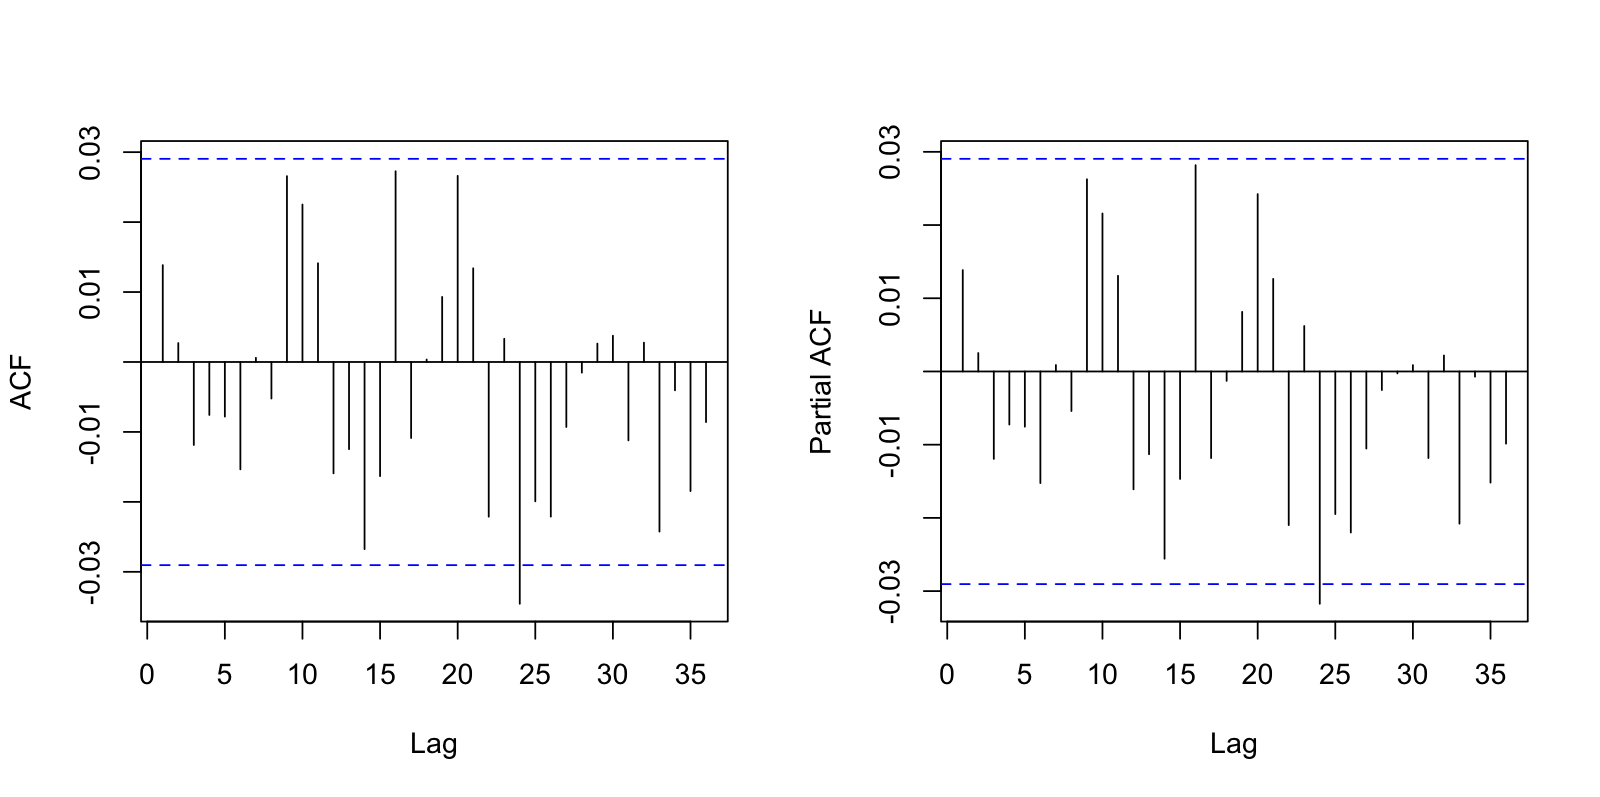
\includegraphics[width=0.85\linewidth]{content/plots/acf_pacf_std_resid.png}
	\caption{ACF and PACF of the Standard Residuals of GARCH(1,1) with ARMA(0,2) mean}
	\label{fig:acf_pacf_std_resid}
\end{figure}


Figure (\ref{fig:acf_pacf_std_resid}) shows the ACF/PACF standard residuals from GARCH(1,1) with ARMA(0,2) mean. The ACF plot shows that most autocorrelations are within the significance bounds, with only a few minor expects (lag 5). Otherwise, there are no systematic patterns of significant autocorrelation across lags. The PACF again shows a significant spike at lag 5, but all other lags fall within the confidence bounds. The lack of significant autocorrelation in both plots suggest that the ARMA(0,2) specification has adequately captured the linear dependence in the means of QCOM. The isolated spikes at lag 5 are likely due to random noise rather than model misspecification.

Figure (\ref{fig:acf_pacf_squared_resid}) shows the ACF/PACF plots for squared residuals of the GARCH(1,1) model. A notable significant spike at lag 1 that clearly exceeds the confidence bounds. We also have some other minor spikes at various lags that approach but mostly stay within the significance boundaries. In terms of the PACF, we have mutliple significant lags at 3. 

\begin{figure}[!h]
	\centering
	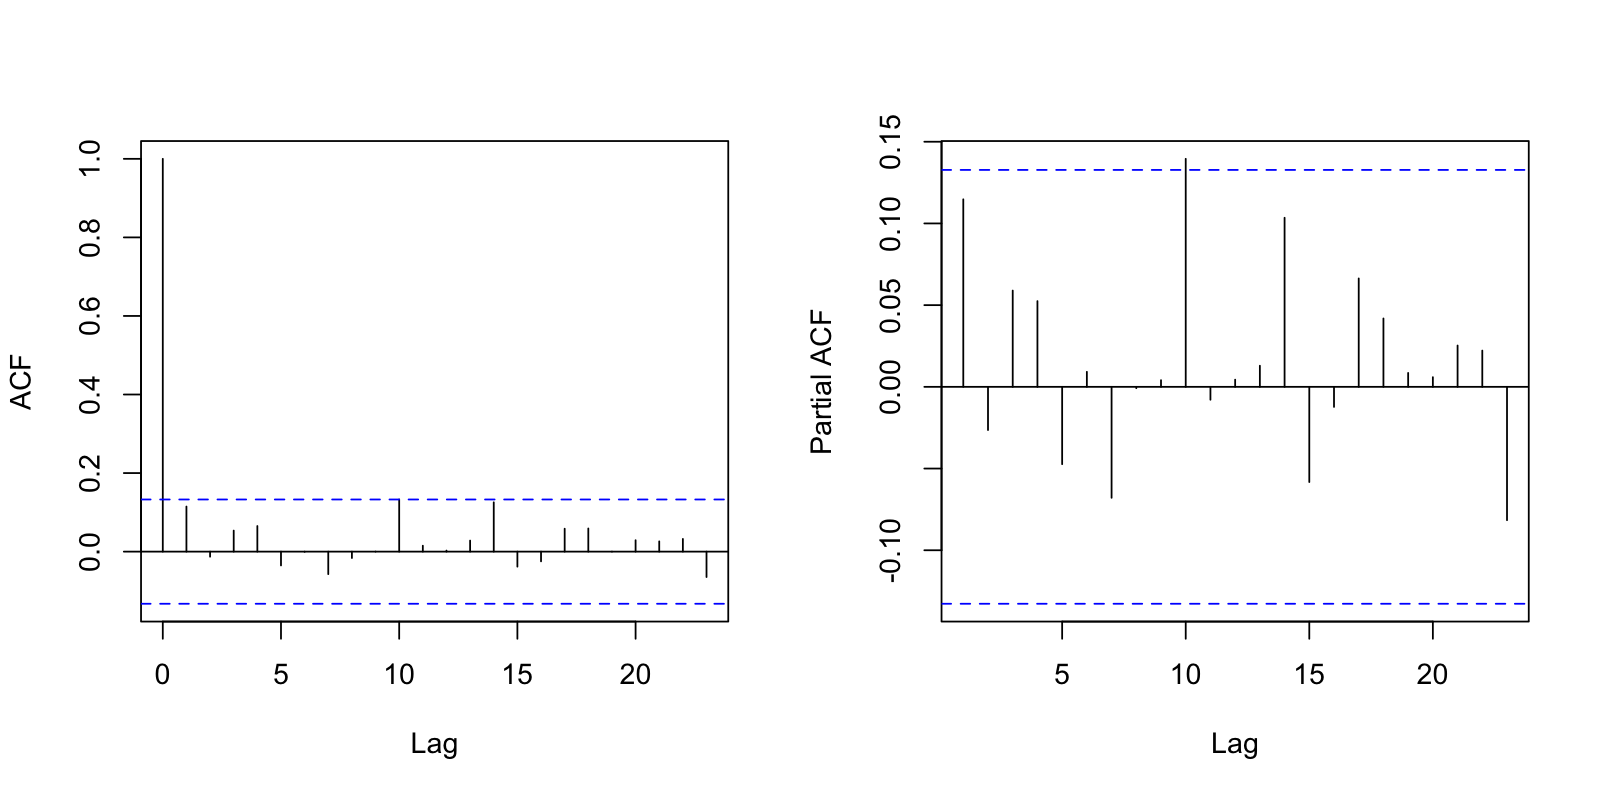
\includegraphics[width=0.85\linewidth]{content/plots/acf_pacf_squared_resid.png}
	\caption{ACF and PACF of the Squared Residuals of GARCH(1,1) with ARMA(0,2) mean}
	\label{fig:acf_pacf_squared_resid}
\end{figure}

This shows that there may be some remaining ARCH effects in the model, and more refinement is necessary.

We find the the optimal GARCH orders by using the EACF, which involves  locating the corner of insignificant autocorrelations (marked o); a similiar process for identifying the optimal ARIMA model. As we can see Table (\ref{tab:eacf_garch}) shows the first clear triangle which starts at AR=1 (GARCH Term) and MA=4 (ARCH term), suggesting a GARCH(1,1) specification, which is our first model of choice. Since higher orders of GARCH will not necessarily improve the model (according to the AIC), we can use extensions of GARCH, such as EGARCH and and GJR-GARCH.

\begin{table}[H]
	\centering
	\caption{Extended Autocorrelation Function (EACF) for QCOM Log Returns}
	\begin{tabular}{c|cccccccccccccc}
		$(p, q)$ & 0 & 1 & 2 & 3 & 4 & 5 & 6 & 7 & 8 & 9 & 10 & 11 & 12 & 13 \\
		\hline
0 & o & o & o & o & o & o & o & o & o & o & o & o & o & o \\
1 & x & o & o & o & o & o & o & o & o & o & o & o & o & o \\
2 & x & x & o & o & o & o & o & o & o & o & o & o & o & o \\
3 & x & x & x & o & o & o & o & o & o & x & o & o & o & o \\
4 & x & x & x & x & o & o & o & o & o & o & o & o & o & o \\
5 & x & x & x & x & o & o & o & o & o & o & o & o & o & o \\
6 & x & x & x & o & x & o & o & o & o & o & o & o & o & o \\
7 & o & o & x & o & x & o & o & o & o & o & o & o & o & o \\
		\label{tab:eacf_garch}
	\end{tabular}
\end{table}

\section{GARCH Extension}

\subsection{EGARCH}

The Exponential GARCH (EGARCH) model  is a generalized form of the traditional GARCH model that captures asymmetric volatility responses to shocks in financial time series. Unlike standard GARCH models that impose positivity constraints on parameters to ensure a positive conditional variance, the EGARCH model operates in logarithmic form, guaranteeing positivity without explicit constraints. The EGARCH(1,1) specification is given by the following:

\begin{equation}
	\log\left(\sigma_t^2\right)=\omega+\beta\log\left(\sigma_{t-1}^2\right)+\alpha\left(\frac{|z_{t-1}|}{\sqrt{2/\pi}}-1 \right)+\gamma z_{t-1},
\end{equation}
where $\sigma_t^2$ is the conditional variance, $z_{t-1}=\frac{\epsilon_{t-1}}{\sigma_{t-1}}$ is the standard innocation, and $\omega,\beta,\alpha,$ and $\gamma$ are the model parameters. The term involving $|z_{t-1}|$ captures the magnitudes effect of shocks, while the $\gamma z_{t-1}$ term captures leverage effects allowing negative shocks to have a different impact on volatility than positive ones. This flexibility makes the EGARCH model particularly well-suited for modeling financial returns exhibiting volatility clustering and asymmetric responses to news.

\subsection{GJR-GARCH}

The GJR-GARCH model extends the standard GARCH model to account for asymmetric effects in volatility, often referred to as the leverage effect. In financial time series, negative shocks typically increase future volatility more than positive shocks of the same magnitude. The GJR-GARCH(1,1) model captures this behavior by including an indicator function that activates when the past innovation is negative. The conditional variance equation is given by the following

\begin{equation}
	\sigma_t^2 = \omega + \alpha \epsilon_{t-1}^2 + \gamma \epsilon_{t-1}^2 I_{\{\epsilon_{t-1} < 0\}} + \beta \sigma_{t-1}^2,
\end{equation}
where $\epsilon_{t-1}$ is the previous period's shock, $\sigma_t^2$ is the conditional variance, and $I_{\{\epsilon_{t-1} < 0\}}$ is an indicator function that equals 1 when $\epsilon_{t-1} < 0$ and 0 otherwise. The parameters $\omega > 0$, $\alpha \geq 0$, $\beta \geq 0$, and $\gamma \geq 0$ determine the dynamics of the model. The presence of $\gamma$ allows the model to respond more aggressively to negative shocks, thus capturing the asymmetry in financial return volatility.

\section{IGARCH}

The Integrated GARCH (IGARCH) model is a special case of the GARCH model where the effect of past shocks on current volatility does not decay over time. In particular, the sum of the ARCH and GARCH parameters equals one, implying a unit root in the conditional variance equation. The IGARCH(1,1) model is specified as by the following:

\begin{equation}
	\sigma_t^2 = \omega + \alpha \epsilon_{t-1}^2 + (1 - \alpha) \sigma_{t-1}^2,
\end{equation}
where $\omega \geq 0$, $0 \leq \alpha \leq 1$, and the constraint $\alpha + \beta = 1$ is imposed (with $\beta = 1 - \alpha$). This structure implies that shocks to volatility are persistent and have long-lasting effects, a common feature in high-frequency financial return data. Because the variance is integrated (non-stationary), the IGARCH model is typically used to model processes with permanent volatility dynamics and is often applied when testing for unit roots in volatility or as an intermediate step before fitting more flexible models like FIGARCH.

\section{TGARCH}

The Threshold GARCH (TGARCH) model introduces asymmetry in the conditional variance by allowing the impact of positive and negative shocks to differ. Unlike standard GARCH models, the TGARCH specification models the conditional standard deviation (rather than variance), making the asymmetry directly interpretable in terms of volatility. The TGARCH(1,1) model is expressed as:

\begin{equation}
	\sigma_t = \omega + \alpha |\epsilon_{t-1}| + \gamma \epsilon_{t-1} I_{\{\epsilon_{t-1} < 0\}} + \beta \sigma_{t-1},
\end{equation}
where $\epsilon_{t-1}$ is the previous shock, $\sigma_t$ is the conditional standard deviation, and $I_{\{\epsilon_{t-1} < 0\}}$ is an indicator function equal to 1 when the shock is negative. The parameter $\gamma$ captures the asymmetric response of volatility to negative shocks—allowing volatility to rise more in response to bad news than to good news of the same magnitude. This formulation makes TGARCH especially suitable for modeling the leverage effect observed in financial markets.
\section{Model Selection }

Table (\ref{tab:GARCH_model}) show that the best extension of GARCH is the EGARCH 

\begin{equation}
\begin{aligned}
	r_t &= \mu + \phi_1 r_{t-1} + \phi_2 r_{t-2} + \theta_1 \epsilon_{t-1} + \theta_2 \epsilon_{t-2} + \epsilon_t \\
	& = 0.006454 + 0.028517 r_{t-1} + 0.807257 r_{t-2} - 0.198846 \epsilon_{t-1} - 0.875843 \epsilon_{t-2}
\end{aligned}
\end{equation}
where $r_t$ is the value of the time series at time $t$, $\mu$ is the constant term, $\phi_1$ and $\phi_2$ are the autoregressive coefficients for the first and seceond lags of $r_t$, $\theta_1$ and $\theta_2$ are the moving average coefficients for the first and second lags of the error term $\epsilon_t$

\begin{equation}
	\begin{aligned}
		\sigma_t^2 &= \omega + \alpha_1 \epsilon_{t-1}^2 + \beta_1 \sigma_{t-1}^2 \\
		&= -0.770193 - 0.184622 \epsilon_{t-1}^2 - 0.011050 I_{t-1} \epsilon_{t-1}^2 + 0.842590 \sigma_{t-1}^2
	\end{aligned}
\end{equation}


where $\sigma_t^2$ is the conditional variance at time $t$, $\omega$ is the constant term in the variance equation, $\alpha_1$ is the ARCH parameter, which measures the reaction to conditional variance to past shocks, and $\beta_1$ is the GARCH parameter, which measures the persistence of the conditional variance based on past conditional variances. We also have 

\begin{itemize}
	\item $I_{t-1} = 1$ if $\epsilon_{t-1} < 0$ (negative shock)
	\item $I_{t-1} = 0$ if $\epsilon_{t-1} \geq 0$ (positive shock)
\end{itemize}
The mean dynamics show minimal first-order autoregression (0.029) but strong second-order effects (0.807), suggesting momentum effects with a two-period lag. The significant negative moving average terms (-0.199 and -0.875) indicate complex error correction mechanisms where past shocks have persistent negative effects on current returns.

The variance equation exhibits strong volatility persistence ($\beta_1$ = 0.843), but lacks significant asymmetric response to negative shocks ($\gamma_1$ = -0.011, $p = 0.930$). The negative constant term ($\omega$ = -0.770) and ARCH parameter ($\alpha$ = -0.185) are unconventional and require careful interpretation, as negative values in the variance equation could potentially lead to negative conditional variance predictions under certain conditions. The Student’s t-distribution with approximately 5.7 degrees of freedom accommodates the fat-tailed nature of financial returns, capturing extreme market movements better than a normal distribution would.

The variance equation exhibits strong volatility persistence ($\beta_1$= 0.843), but lacks significant asymmetric response to negative shocks ($\gamma_1$ = -0.011, $p$ = 0.930). The negative constant term ($\omega$ = -0.770) and ARCH parameter ($\alpha_1$ = -0.185) are unconventional and require careful interpretation, as negative values in the variance equation could potentially lead to negative conditional variance predictions under certain conditions. The Student’s t-distribution with approximately 5.7 degrees of freedom accommodates the fat-tailed nature of financial returns, capturing extreme market movements better than a normal distribution would.

\section{Forecasting}

\begin{figure}[!h]
	\centering
	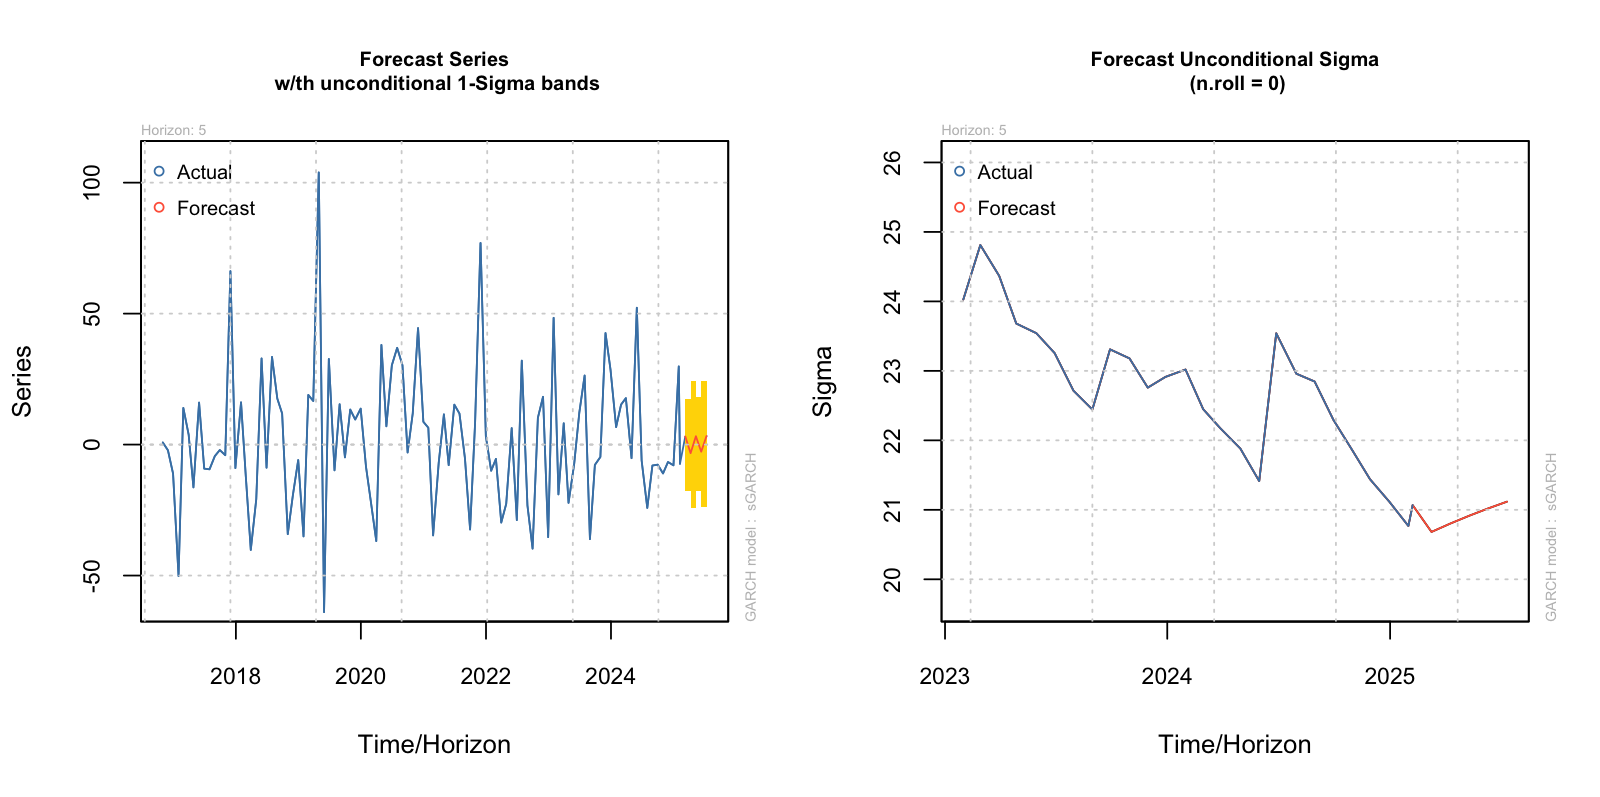
\includegraphics[width=0.85\linewidth]{content/plots/GARCH_forecast.png}
	\caption{ACF and PACF of the Squared Residuals of EGARCH(1,1)}
	\label{fig:GARCH_forecast}
\end{figure}

Figure (\ref{fig:GARCH_forecast}) shows the forecast for the EGARCH(1,1), which provides valuable insights into both the predicted returns and volatility patterns. The left panel displays the historical series (blue line) characterized by significant fluctuations over the 2018-2025 period, with several dramatic spikes exceeding 50 units in both positive and negative directions. The forward-looking forecast (orange line) projects relatively modest returns with a slight upward trend, accompanied by widening yellow confidence bands that reflect increasing uncertainty over the 5-period forecast horizon. This suggests that while the model anticipates positive returns in the near future, it acknowledges considerable uncertainty in these predictions, consistent with the historical volatility observed in the series.

The right panel, displaying unconditional sigma (volatility) forecasts, reveals that volatility has followed a generally declining trend from about 24.5 units in early 2023 to approximately 20.7 units by early 2025. The model forecasts a modest uptick in volatility over the next five periods. This slight increase in projected volatility aligns with the expanding confidence intervals seen in the returns forecast. The overall pattern suggests that while the EGARCH model expects volatility to remain lower than historical peaks, it anticipates some volatility persistence - a typical characteristic of financial time series modeled with EGARCH specifications. This measured increase in forecasted volatility indicates the model’s response to recent market conditions, though the magnitude remains relatively contained compared to historical levels.

